\documentclass[DIV=15, titlepage,10pt]{scrartcl}
\usepackage{graphicx} % Für die Bilder zum Schwerpunkt
% \usepackage[utf8]{inputenc} % Für Umlaute
\usepackage[german]{babel} 
\usepackage{amsmath}
\usepackage{amssymb}
\usepackage{pgfplots}
\usepackage{subcaption}

\begin{document}

\title{Aufgabe 1}
\subtitle{Gruppe 4}
\author{
  Jonas Eckhoff
  \and
  Anton Jabs
  \and
  Florian Brach
  \and
  Felix Kieckhäfer
}

\publishers{%
    \normalfont\normalsize%
    \parbox{0.8\linewidth}{%
      Zur Regelauslegung in der Simulationsumgebung wird ein genaues Farzeugmodell benötigt. Dafür müssen unter anderem unbekannte Systemparameter gemessen werden. Je genauer diese bestimmt werden, desto besser kann die Dynamik modelliert werden. Im Nachfolgenden werden vier Versuche beschrieben, die wir durchgeführt haben um die unbekannten Parameter zu bestimmen. 
    }
}

% \begin{abstract}
% Zur Regelauslegung in der Simulationsumgebung wird ein genaues Farzeugmodell benötigt. Dafür müssen unter anderem unbekannte Systemparameter gemessen werden. Je genauer diese bestimmt werden, desto besser kann die Dynamik modelliert werden. Im Nachfolgenden werden vier Versuche beschrieben, die wir durchgeführt haben um die unbekannten Parameter zu bestimmen. 
% \end{abstract}

\maketitle[0]




\section{Die Bilderkennung}

Das Ziel der Bilderkennung ist es, zwei Punkte zu identifizieren, von denen man den Abstand in den Weltkoordinaten kennt. Anschließend kann man dann durch eine Koordinatentransformation von den Bildkoordinaten zu den Weltkoordinaten die Position der Kamera in der Welt in Relation zum bekannten Objekt bestimmen. Für dieses Objekt haben wir ein rotes Rechteck gewählt.

\subsection{Bildvorverarbeitung}

Zuerst soll das Bild so angepasst werden, dass das rote Rechteck einfacher identifizierbar wird. 
Normalerweise würde man damit beginnen, das Bild erstmal vorzuglätten (zum Beispiel mit einem Gauss-Filter) um Rauschen zu minimieren. Dies hat sich aber aus Performancegründen als nicht so hilfreich herausgestellt. Stattdessen kann hier gut die Eigenschaft, dass das Rechteck rot ist, verwendet werden. Wenn man sich die RGB-Kanäle (a, b und c) anschaut, fällt auf, dass das rote Rechteck sehr hell im roten Kanal ist, allerdings fast gar nicht in dem blauen und grünen Kanal sichtbar ist. Alle anderen Farben haben auch einen Blau- oder Grünanteil. Aus diesem Grund wird im ersten Schritt ein Graustufenbild (e) erzeugt, in dem der blaue und grüne Kanal vom roten Kanal abgezogen werden.

\begin{center}
\begin{table}[ht]
\begin{tabular}{c c c}
\begin{subfigure}{0.3\textwidth}\centering

\includegraphics[scale=0.08]{Figures/rotkanal.png} \vspace{-3.5mm}\caption{Rotkanal}
\end{subfigure}&
\begin{subfigure}{0.3\textwidth}\centering

\includegraphics[scale=0.08]{Figures/gruenkanal.png} \vspace{-3.5mm}\caption{Grünkanal}
\end{subfigure}&\begin{subfigure}{0.3\textwidth}\centering

\includegraphics[scale=0.08]{Figures/blaukanal.png} \vspace{-3.5mm}\caption{Blaukanal}
\end{subfigure}\\ 
\begin{subfigure}{0.3\textwidth}\centering

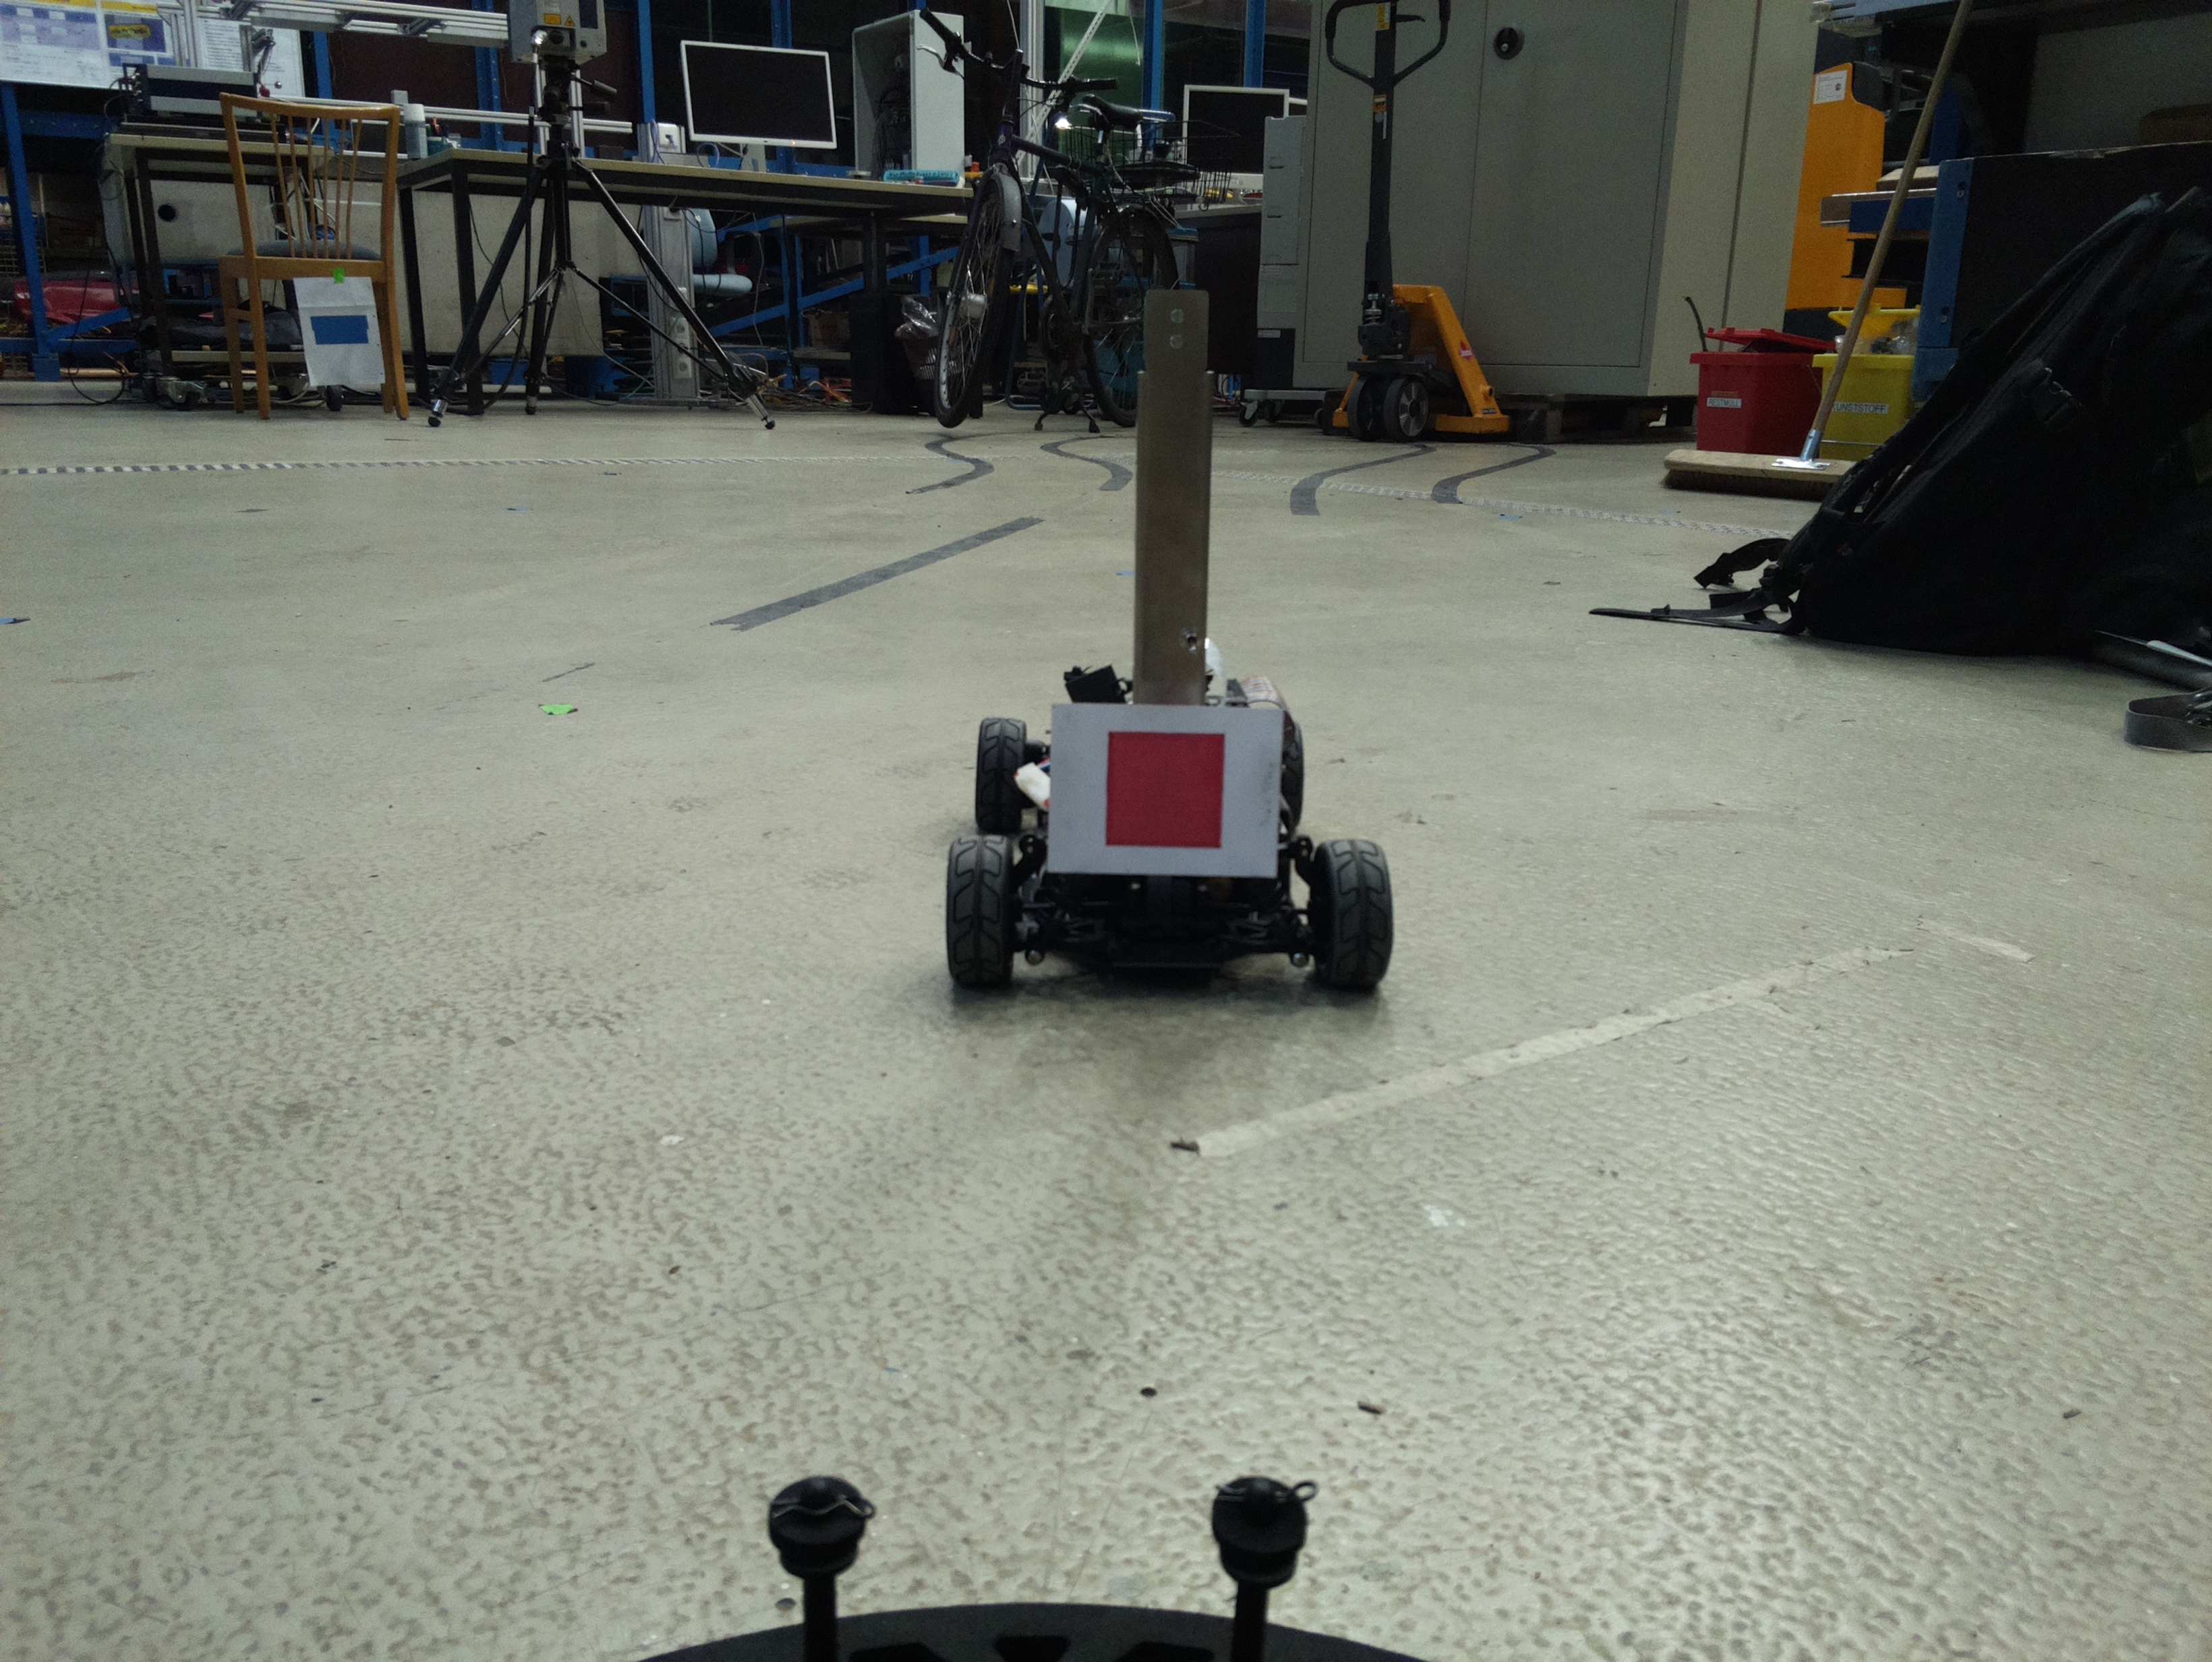
\includegraphics[scale=0.08]{Figures/rechteckbild.png} \vspace{-3.5mm}\caption{Farbbild}
\end{subfigure}&\begin{subfigure}{0.3\textwidth}\centering

\includegraphics[scale=0.08]{Figures/r-g-b.png}  
\vspace{-3.5mm}\caption{Rot-0.5(Grün+Blau)}
\end{subfigure}&\begin{subfigure}{0.3\textwidth}\centering

\includegraphics[scale=0.08]{Figures/binaerbild.png} \vspace{-3.5mm}\caption{Binärbild}
\end{subfigure}
\end{tabular}
\end{table}
\end{center}
\vspace{-5mm}

In diesem Graustufenbild (e) sind nun hauptsächlich helle Rottöne sichtbar. Nun kann ein Binärbild (f) erstellt werden, indem alle Grautöne über einem Schwellenwert weiß dargestellt werden und alle anderen schwarz. 


\subsection{Rechteckserkennung}

Nun sollen die Eckpunkte des Rechteckes gefunden werden. Im ersten Schritt wird ein Gitter über das Bild gelegt, das so fein gewählt wird, dass ein Gitterpunkt auf jeden Fall im Rechteck liegen muss. Dafür wird angenommen, dass das Rechteck eine Mindestgröße im Bild hat und nicht zu weit weg ist. Ob ein Gitterpunkt $(x_1,y_1)$ nun wahrscheinlich in einem Rechteck liegt, wird mithilfe des Algorithmus 1 festgestellt.\\


\begin{figure*}[h]
  \centering
\begin{minipage}[t]{0.5\textwidth}
\centering
\vspace{-0.4cm}
\renewcommand\figurename{Algorithm}
\begin{algorithm}[H]
\caption{Pseudo-Code}\label{euclid}
\begin{algorithmic}[1]
\State $(x,y) = (x_1, y_1)$
\While {$I(x,y) = $ white}
	\State $ y = y - 1$
\EndWhile

\State $ y_2 = y$
\State $(x,y) = (x_1, y_1)$
\While {$I(x,y) = $ white}
	\State $ y = y + 1$
\EndWhile
\State $y_3 = y$
\end{algorithmic}
\end{algorithm}

\end{minipage}\hfill
  \begin{minipage}[t]{0.35\textwidth}
    \centering
    \raisebox{-\height}{\includegraphics[width=1\textwidth]{Figures/rechteckgrafik.pdf}}
    \vspace{-0.2cm}
    \caption{Beispiel-Rechteck}\label{fig:xx}
  \end{minipage}\hfill

\end{figure*}
%
Dies bestimmt den Punkt $(x_1,y_2)$ und $(x_1,y_3)$. 
Anschließend lässt sich der Mittelpunkt {$(x_1,y_m)=(x_1,\frac{y_2+y_3}{2})$ bestimmen. Nun wird der gleiche Algorithmus nochmal in x-Richtung durchgeführt mit Startwert $(x_1,y_m)$ um $x_l$ und $x_r$ zu finden. Um leicht schräge Seiten auszugleichen, wird nun der Algorithmus auf $(x_l+a,y_m)$ und $(x_r-a,y_m)$ angewandt, um die die vier Rechtecksecken $(x_{ol},y_{ol}),(x_{or},y_{or}),(x_{ul},y_{ul})$ und $(x_{ur},y_{ur}))$ zu finden.\\
%
Nun wird noch überprüft, ob die gefundenen Ecken ein sinnvolles Rechteck bilden. Dafür darf $y_{ol}-y_{ul}$ nicht mehr als $ 30\% $ größer oder kleiner als $y_{or}-y_{ur}$ oder $x_r-x_l$ sein, da das Rechteck leicht nach hinten gekippt sein kann (vorausfahrendes Auto lenkt). Außerdem soll noch $\frac{y_m-y_{ol}}{y_m-y_{or}}$ ungefähr $\frac{y_{ul}-y_{m}}{y_{ur}-y_{m}}$ sein. Wenn diese Bedingungen eingehalten werden, handelt es sich wahrscheinlich um ein Rechteck.\\
%
Um möglichst schnell den richtigen Startpunkt $(x_1,y_1)$ zu finden, wird spiralförmig um den Mittelpunkt des im letzten Bild gefundenen Rechtecks gesucht.

\section{Massenträgheitsmoment}
\subsection{Theorie}
Das Trägheitsmoment kann experimentell durch einen Pendelversuch bestimmt werden. 
Für eine harmonische Schwingung kann die Auslenkung $x$ mit der Kreisfrequenz $\omega$ als Funktion der Zeit dargestellt werden:
\[ \frac{d^2x}{dt^2}+\omega^2x=0.\]
Das Drehmoment, das auf den Körper wirkt beträgt 
\[M=-mgd = -mglsin(\varphi).\]
In Verbindung mit \(M(t) = I\alpha(t)\) gilt \[ \frac{d^2\varphi}{dt^2}+\frac{mgl}{I}sin(\varphi)=0.\]
Für kleine Winkel und der damit verbundenen Annahme \(sin(\varphi)\approx \varphi\) gilt \[\frac{d^2\varphi}{dt^2}+\frac{mgl}{I} \varphi =0.\]
Damit ist  die Schwingungsdauer $T$  
\[T=\frac{2\pi}{\omega} = 2\pi \sqrt{\frac{I}{mgl}}\] 
und das Trägheitsmoment $I$ 
\[I=\Big(\frac{T}{2\pi}\Big)^2mgl.\]

\subsection{Praxisversuch}
Das für den Pendelversuch verwendete Pendel besteht aus einer Holzplatte und einem Gestell. Das kombinierte Trägheitsmoment für Platte und Gestell bezüglich des gemeinsamen Schwerpunktes beträgt $0.057 kg m^2.$
Die Schwingungsdauer $T$ mit montiertem Auto beträgt $1.3749s$, das Gesamtgewicht aus Holzplatte, Gestell und Auto ergibt sich zu $m_{ges}=0.846+1.152+2.26 = 4.258kg$. Die Pendellänge $l$ ist der Abstand  vom gemeinsamen Schwerpunkt zur Drehachse und beträgt  $0.383m.$   Daraus  ergibt sich ein Trägheitsmoment von 
\[I_{ges} = \Big(\frac{1.3749 s}{2\pi}\Big)^2 \cdot 4.258 kg \cdot 9.81\frac{m}{s^2} \cdot 0.383m = 0.7662 kg m^2.\]
Dieses ist das Trägheitsmoment  des kombinierten Körpers (Holzplatte, Gestell und Auto) bezüglich der Drehachse. Mit Hilfe des Steiner'schen Satzes kann die Bezugsachse in den gemeinsamen Schwerpunkt verschoben werden: 
\[I_{ges,SP} = I_{ges} + m_{ges} \cdot l^2  \hspace{5mm} \rightarrow  \hspace{5mm} 0.7662 kg m^2+ 4.258 kg \cdot (0.383m)^2 = 1.39kgm^2.\] 
Das Trägheitsmoment des Autos bezüglich des Schwerpunkts berechnet sich aus der Differenz des Gesamtträgheitsmoment und des Trägheitsmoment der Aufhängung:
\[1.39kgm^2-0.057kgm^2 = 1.333 kgm^2.\]

\section{Beziehung von Stellgrößen der Motoren zu Lenkwinkel und Geschwindigkeit}
\section{Über-/Untersteuerung und Seitenkraftbeiwerte}

\end{document}